
\documentclass[a4paper,10pt]{article}

\usepackage{graphicx}
\begin{document}


\section{How the model progressed}
Figures 2, 3, 4, and 5 in section shows blueprints of each deck: Weather Deck, Tween Deck, Lower Deck and Cargo Hold respectively.
\begin{center}
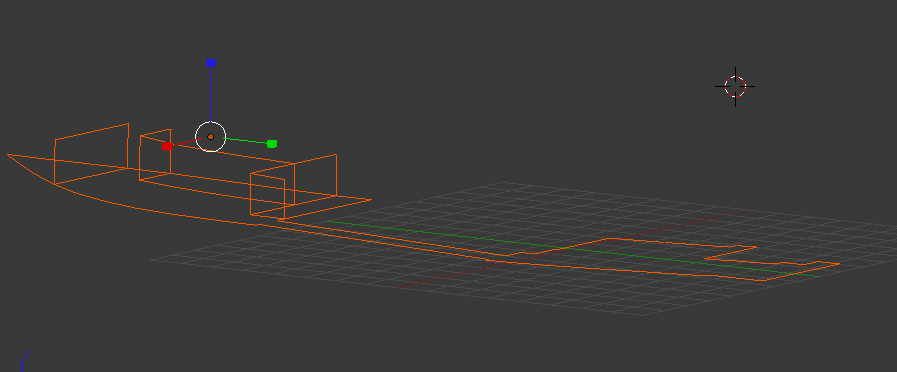
\includegraphics[scale=0.5]{../images/deck.png}
\\layer of deck
\end{center}
Each blueprint is used as a model to build a ship starting from the lowest to top deck and it is modelled individually using Blender layer.
To make curvatures matched to the floors accurately, cross sectionals is used so model scaling can be seen easily.
It is difficult to model a ship hull using only cross sectionals because its shape is round and consists of two or more profiles.
Therefore, skinning is applied (the fine art of defining a surface using more than one profiles).
In blender, skinning can be adopted by preparing as many curves of the desired shape and then converting them to a single NURBS(Non-Uniform Rational B-Spline) 
surface.
\end{document}


